% Reporte del modelo AgroCebada. Formato IEEEtran con portada propia.
% Compilar desde docs/reporte_modelo (dos veces, para las referencias cruzadas):
%   xelatex -interaction=nonstopmode main.tex && xelatex -interaction=nonstopmode main.tex
% IEEEtran.cls, algorithmicx.sty y algpseudocode.sty van en esta carpeta porque no vienen en el TeX Live instalado.
\documentclass[conference,letterpaper]{IEEEtran}
\usepackage{fontspec}
\setmainfont{TeX Gyre Termes}
\usepackage{polyglossia}
\setdefaultlanguage{spanish}
\usepackage{amsmath,amssymb}
\usepackage{graphicx}
\usepackage{booktabs}
\usepackage{array}
\usepackage{xcolor}
\usepackage[caption=false,font=footnotesize]{subfig}
\usepackage{algorithm}
\usepackage[noend]{algpseudocode}
\usepackage{tikz}
\usetikzlibrary{positioning,arrows.meta}
\usepackage{hyperref}
\hypersetup{colorlinks=true,linkcolor=black,citecolor=black,urlcolor=blue!50!black}
\graphicspath{{figuras/}}

% Pseudocódigo en español.
\floatname{algorithm}{Algoritmo}
\algrenewcommand\algorithmicfunction{\textbf{función}}
\algrenewcommand\algorithmicprocedure{\textbf{procedimiento}}
\algrenewcommand\algorithmicif{\textbf{si}}
\algrenewcommand\algorithmicthen{\textbf{entonces}}
\algrenewcommand\algorithmicelse{\textbf{si no}}
\algrenewcommand\algorithmicfor{\textbf{para cada}}
\algrenewcommand\algorithmicdo{\textbf{hacer}}
\algrenewcommand\algorithmicloop{\textbf{repetir}}
\algrenewcommand\algorithmicreturn{\textbf{devolver}}
\algrenewcommand\alglinenumber[1]{\footnotesize #1}
\algrenewcommand{\algorithmiccomment}[1]{\hfill{\footnotesize\textit{// #1}}}

\newcommand{\code}[1]{\texttt{#1}}

% ---------------------------------------------------------------- datos de la portada
\newcommand{\universidad}{Benemérita Universidad Autónoma de Puebla}
\newcommand{\facultad}{Facultad de Ciencias de la Computación}
\newcommand{\carrera}{Reto AgroCebada FIRA 2026}
\newcommand{\materia}{Reporte técnico del modelo}
\newcommand{\integranteA}{José Alán Pomares Valdés}
\newcommand{\integranteB}{Luis Emmanuel Ramiro Luna}
\newcommand{\integranteC}{Vicente Josimar López Martinez}
\newcommand{\correo}{pv202351433@alm.buap.mx}
\newcommand{\asesor}{Luis Gustavo Olivares Soto}
\newcommand{\fecha}{7 de octubre de 2026}

% Encabezado de la portada. Si existen figuras/logo_buap.png y figuras/logo_fcc.png se usan, si no queda un recuadro.
\newcommand{\logo}[2]{%
  \IfFileExists{figuras/#1}{\includegraphics[height=2.4cm]{#1}}%
  {\fbox{\parbox[c][2.2cm][c]{2.2cm}{\centering\footnotesize\textcolor{gray}{#2}}}}}

\begin{document}

% ---------------------------------------------------------------- portada
\begin{titlepage}
  \centering
  \begin{tabular}{@{}m{2.6cm}@{}m{\dimexpr\textwidth-5.2cm}@{}m{2.6cm}@{}}
    \logo{logo_buap.png}{Logo BUAP} &
    \centering{\Large\bfseries \universidad}\\[4pt]{\large \facultad} &
    \hfill\logo{logo_fcc.png}{Logo FCC}
  \end{tabular}\par
  \vspace{4pt}\rule{\textwidth}{1.2pt}\par
  \vspace{1.2cm}
  {\large \carrera}\par\vspace{4pt}
  {\large \materia}\par
  \vspace{3cm}
  {\Huge\bfseries Rendimiento de cebada de temporal\\[6pt] con régimen de etiquetas\\[6pt] y rezago espacial}\par
  \vspace{0.8cm}
  {\Large Procedimiento, arquitectura y evaluación del modelo}\par
  \vfill
  \begin{tabular}{@{}r@{\hspace{1em}}l@{}}
    \textbf{Integrantes} & \integranteA \\
                         & \integranteB \\
                         & \integranteC \\[4pt]
    \textbf{Asesor}      & \asesor \\[4pt]
    \textbf{Contacto}    & \href{mailto:\correo}{\correo} \\
  \end{tabular}\par
  \vspace{1.5cm}
  {\large Puebla, Pue., \fecha}\par
\end{titlepage}

\noindent\textbf{\textit{Resumen.}} \bfseries Estimamos el rendimiento de cebada de temporal de 59 parcelas con un
proceso gaussiano que usa dos datos de cada parcela, el régimen de su etiqueta y el rendimiento de sus vecinas del
mismo régimen. Las etiquetas se dividen por municipio en dos formatos con medias de 4.49 y 3.05\,t/ha, y conocer el
formato explica la mayor parte de lo que se puede explicar. Construimos el modelo paso a paso. Cada idea entró solo si
mejoraba la validación cruzada de forma consistente y pasaba una prueba de permutación. Así quedaron fuera las
variables satelitales, climáticas y topográficas, que no mejoraron la predicción una vez conocidos el régimen y los
vecinos. El modelo obtiene un RMSE de 0.458\,t/ha en validación cruzada, contra 0.489 de la media por régimen. Como el
modelo se eligió entre muchas variantes, estimamos con validación anidada un RMSE esperado de 0.46 a 0.49\,t/ha.\par\mdseries

\smallskip
\noindent\textbf{\textit{Palabras clave.}} \bfseries rendimiento de cebada, régimen de etiquetas, rezago espacial,
proceso gaussiano, validación cruzada, predicción conformal.\par\mdseries

\section{Introducción}\label{sec:intro}

El reto AgroCebada de FIRA 2026 pide estimar el rendimiento de cebada de temporal, en toneladas por hectárea (t/ha),
de 59 parcelas de Hidalgo, Puebla y Tlaxcala. Estas tres entidades se cuentan entre las cuatro principales productoras
de cebada grano del país~\cite{sader2025}. Para entrenar tenemos 138 parcelas del mismo ciclo de 2025 con su
rendimiento declarado, imágenes de los satélites Sentinel-2~\cite{drusch2012} y PlanetScope~\cite{frazier2021},
clima~\cite{funk2015,verdin2020} y topografía. El jurado califica primero el error de las 59 predicciones con el RMSE,
que se mide en t/ha y castiga más los errores grandes.

La predicción de rendimiento con aprendizaje automático y teledetección es un tema muy estudiado~\cite{vanklompenburg2020,weiss2020}.
En este reto las parcelas son pequeñas y su rendimiento es declarado, no medido, y la literatura reporta que ese tipo
de dato contiene error considerable~\cite{lobell2020}. Por eso el reporte se centra en qué información aporta de
verdad a la predicción y en qué tan confiable es el error que estimamos.

Este reporte explica cómo construimos el modelo y por qué tomamos cada decisión. La Fig.~\ref{fig:flujo} resume el
proceso. Partimos de un hallazgo en las etiquetas (Sección~\ref{sec:datos}), fijamos cómo íbamos a evaluar cada idea
(Sección~\ref{sec:evaluacion}) y agregamos piezas una por una, conservando solo las que mejoraban la validación
(Sección~\ref{sec:construccion}). Después describimos el modelo final (Sección~\ref{sec:final}), qué tan confiable es
su error (Sección~\ref{sec:confiabilidad}) y qué aportan los índices satelitales (Sección~\ref{sec:indices}).

\begin{figure*}[t]
\centering
\begin{tikzpicture}[node distance=0.45cm, every node/.style={font=\footnotesize, align=center},
  caja/.style={draw=black!60, rounded corners=2pt, minimum height=1.05cm, text width=2.35cm, fill=black!3},
  clave/.style={caja, draw=blue!60!black, fill=blue!6}, flecha/.style={-{Stealth[length=2mm]}, black!60}]
\node[caja] (d) {Datos\\138 + 59 parcelas\\satélite, clima, suelo};
\node[caja, right=of d] (v) {91 variables\\por parcela};
\node[clave, right=of v] (r) {Régimen de la\\etiqueta (A o B)};
\node[clave, right=of r] (z) {Rezago espacial\\vecinos a 400\,m};
\node[clave, right=of z] (g) {Proceso\\gaussiano};
\node[caja, right=of g] (s) {Predicción\\e intervalo\\p10 a p90};
\draw[flecha] (d) -- (v); \draw[flecha] (v) -- (r); \draw[flecha] (r) -- (z); \draw[flecha] (z) -- (g); \draw[flecha] (g) -- (s);
\node[below=0.25cm of v, text width=2.6cm, font=\scriptsize, text=black!60] {probadas, sin mejora\\(Sección~\ref{sec:bloques})};
\end{tikzpicture}
\caption{Arquitectura del modelo. En azul, las piezas que usa el modelo final. Las 91 variables satelitales, de clima
y de topografía se probaron una por bloque y ninguna mejoró la validación.}
\label{fig:flujo}
\end{figure*}

\section{Datos y el hallazgo de los regímenes}\label{sec:datos}

Hay 197 parcelas en nueve municipios, 138 de entrenamiento y 59 de predicción. FIRA hizo la partición al azar y
estratificada por zona, así que cada municipio con parcelas por predecir también tiene parcelas de entrenamiento. De
las series de tiempo construimos 91 variables por parcela, como el máximo del índice de vegetación NDVI
en 2025, la fenología~\cite{zadoks1974}, la historia de 2022 a 2024, la heterogeneidad dentro de la parcela, el clima y
la topografía. Ninguna usa el rendimiento.

\textbf{Dos maneras de reportar el rendimiento.} Al revisar las etiquetas encontramos dos maneras de reportar el
rendimiento, y cada municipio usa una sola (Fig.~\ref{fig:regimenes}). En cuatro municipios el rendimiento viene con
dos decimales y promedia 4.49\,t/ha. Lo llamamos régimen A. En los otros cinco todos los valores de entrenamiento
tienen un decimal y promedian 3.05\,t/ha. De las 51 etiquetas de este grupo, 44 son múltiplos de 0.5 y las otras 7, de
Singuilucan, solo de 0.1. Lo llamamos régimen B. Por los decimales no sabemos si el rendimiento se midió de forma
distinta o solo se anotó de forma distinta. FIRA nos confirmó que la fuente es mixta, con una comercializadora como
fuente mayoritaria y el productor como la otra, que la báscula no ajusta por humedad y que debemos tratar todos los
registros como una misma variable objetivo. Tampoco conocemos la fuente de cada parcela. Por eso describimos el régimen
como una observación por municipio. La fuente mixta es una posible explicación, pero no podemos confirmarla.

\textbf{Cómo asignamos el régimen.} El régimen es una regla fija por nombre de municipio (Cuadro~\ref{tab:municipios}).
Una vez fijada, no se recalcula en la validación y no usa el rendimiento de la parcela evaluada. No lo asignamos por el
formato de cada etiqueta, porque 7 de las 87 parcelas del régimen A tienen un solo decimal y una regla por formato las
habría mandado al B. Sí fijamos la regla observando las etiquetas de entrenamiento. En seis parcelas de municipios con
una a tres parcelas de entrenamiento (Tepeapulco, Apan, Nanacamilpa y Emiliano Zapata), el régimen se dedujo de su
propia etiqueta y de la cercanía a municipios vecinos con el mismo formato. Sin esas seis parcelas el RMSE de la
validación pasa de 0.458 a 0.464\,t/ha, así que el efecto es pequeño, pero lo reconocemos como un supuesto de diseño.
Las 59 parcelas por predecir pertenecen a municipios que ya tienen al menos una parcela de entrenamiento. El caso más
delicado es el de la parcela de Nanacamilpa, cuyo régimen se apoya en una sola etiqueta.

\begin{table}[t]
\centering
\caption{Parcelas por municipio y régimen.}
\label{tab:municipios}
\footnotesize
\begin{tabular}{@{}llrr@{}}
\toprule
Municipio & Régimen & Entrenamiento & Predicción \\
\midrule
Chignahuapan & A & 71 & 29 \\
Almoloya & A & 10 & 4 \\
Cuautepec de Hinojosa & A & 5 & 4 \\
Tepeapulco & A & 1 & 0 \\
Calpulalpan & B & 30 & 14 \\
Singuilucan & B & 16 & 7 \\
Emiliano Zapata & B & 3 & 0 \\
Apan & B & 1 & 0 \\
Nanacamilpa & B & 1 & 1 \\
\midrule
Total A, B & & 87, 51 & 37, 22 \\
\bottomrule
\end{tabular}
\end{table}

\begin{figure}[t]
\centering
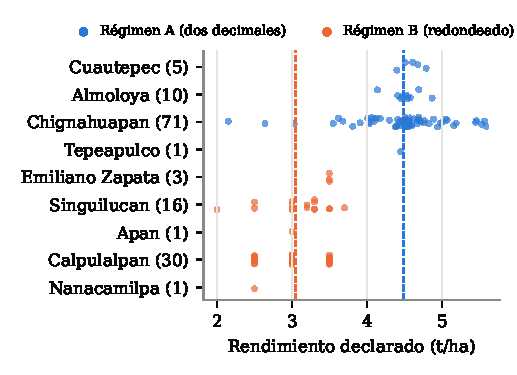
\includegraphics[width=\columnwidth]{f1_regimenes}
\caption{Rendimiento declarado de las 138 parcelas de entrenamiento por municipio, con el número de parcelas entre
paréntesis. Las líneas punteadas son la media de cada régimen.}
\label{fig:regimenes}
\end{figure}

Este hallazgo cambia el problema. La diferencia entre las medias de los regímenes, de 1.4\,t/ha, es casi tres veces la
desviación estándar dentro de cada uno (0.53\,t/ha en A y 0.40 en B). Además, el redondeo de las etiquetas del régimen B
limita lo que cualquier modelo puede predecir. Si el valor verdadero se redondeó a 0.5\,t/ha y se distribuye de forma
uniforme dentro del intervalo de redondeo, el redondeo agrega una desviación de $0.5/\sqrt{12}=0.14$\,t/ha. Esto es una
cota aproximada y no un error mínimo obligatorio, porque 7 de las 51 etiquetas tienen un paso de 0.1. Con la mezcla
observada de pasos la cota es 0.134 y, si todas tuvieran paso de 0.1, sería 0.029. Por el tamaño de la diferencia entre
regímenes, el régimen es la primera pieza del modelo.

\section{Cómo evaluamos cada decisión}\label{sec:evaluacion}

Con 138 parcelas cualquier comparación es ruidosa, así que antes de probar ideas fijamos cómo íbamos a decidir.

\textbf{Error fuera de muestra.} Todas las cifras de RMSE se calculan sobre parcelas que el modelo no vio al
entrenar. Usamos validación cruzada, que reparte las parcelas en 5 grupos (\emph{folds}), entrena con 4 y predice el
quinto, hasta predecir todas. Todo lo que usa el rendimiento, como el rezago espacial, se recalcula dentro de cada
fold para que la parcela evaluada nunca influya en su propia predicción.

\textbf{Dos esquemas.} El esquema A sortea los folds al azar, estratificados por municipio, y repite el sorteo 10
veces. Imita la partición oficial y es el que decide. El esquema B deja fuera zonas completas, uniendo las parcelas a
menos de 2\,km~\cite{roberts2017,ploton2020}, porque la validación al azar tiende a ser optimista cuando hay
autocorrelación espacial. Mide qué tanto depende un modelo de tener vecinos en el entrenamiento.

\textbf{Regla de decisión.} Una idea se acepta si baja el RMSE en al menos 7 de las 10 repeticiones del esquema A y si
pasa una prueba de permutación~\cite{ojala2010}. En esa prueba revolvemos al azar las variables nuevas, dentro de cada
régimen, y repetimos la validación 50 veces con 3 repeticiones cada una. Si el modelo con las variables revueltas
predice igual de bien, la mejora no viene de esas variables y la idea se rechaza. El valor $p$ es la fracción de
permutaciones, contando la real, que predice al menos tan bien como el modelo real. Exigimos $p\le0.05$. Con 50
permutaciones el $p$ más pequeño posible es $1/51=0.0196$, de modo que un valor de 0.02 es el piso de la prueba y no una
medición precisa.

\textbf{Cuántas pruebas hicimos.} Registramos 73 evaluaciones. De ellas, 13 fueron informativas, como las bases de
comparación. Las otras 60 se sometieron a la comparación emparejada por repetición, 10 ganaron en al menos 7
repeticiones y llegaron a la prueba de permutación, y 7 quedaron aceptadas. No corregimos por comparaciones múltiples,
así que los valores $p$ no deben leerse como probabilidades exactas. Con la corrección de Holm solo sobreviven las dos
pruebas de que el régimen supera al estado y al municipio, con $p=0.005$ obtenido con 200 permutaciones. Con el
procedimiento de Benjamini y Hochberg~\cite{benjamini1995}, que controla la tasa de falsos descubrimientos al 5\,\%,
sobreviven cuatro pruebas, las dos anteriores, el rezago espacial y la elección del proceso gaussiano, todas con
$p\le0.0196$. Las tres pruebas con $p=0.039$ no sobreviven. Por esta razón añadimos al final la validación anidada.

\textbf{Controles del resultado final.} Elegir el mejor entre muchos modelos con las mismas particiones infla su
resultado~\cite{cawley2010}. Por eso al final medimos el error esperado con validación anidada~\cite{varma2006},
comparamos modelos con una prueba $t$ corregida por el traslape entre repeticiones~\cite{nadeau2003} y revisamos que
no hubiera fuga de información revolviendo las etiquetas~\cite{kaufman2012}. Estos controles están en la
Sección~\ref{sec:confiabilidad}.

\section{Construcción del modelo}\label{sec:construccion}

Agregamos las piezas en orden, de la más sencilla a la más compleja. Cada pieza tuvo que ganarle a la mejor versión
aceptada hasta ese momento.

\subsection{Punto de partida, la media por régimen}
El modelo más simple predice para cada parcela la media de su grupo. La Fig.~\ref{fig:bases} compara varios grupos.
La media por régimen es la mejor en ambos esquemas, con 0.489\,t/ha. La media por municipio se le acerca en el
esquema A (0.510), pero en el esquema B sube a 0.955 porque, al dejar zonas fuera, muchos municipios se quedan sin
parcelas de entrenamiento. El régimen no tiene ese problema, porque se conoce para cualquier parcela. Por eso es la
base de todo lo demás.

\begin{figure}[t]
\centering
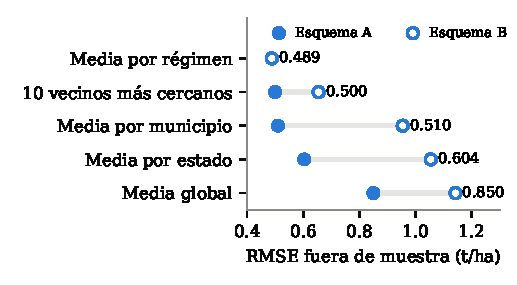
\includegraphics[width=\columnwidth]{f2_bases}
\caption{RMSE de modelos sencillos. El número es el esquema A. La media por régimen es la única que no empeora cuando
se dejan zonas completas fuera (esquema B).}
\label{fig:bases}
\end{figure}

\subsection{Rezago espacial, lo que dicen los vecinos}
Dentro de un régimen el rendimiento todavía varía, y parcelas cercanas tienden a parecerse~\cite{tobler1970}, porque
comparten suelo, clima, manejo y a veces productor. Para aprovecharlo calculamos el \emph{rezago espacial}, el
promedio del rendimiento de las parcelas de entrenamiento cercanas, ponderado por el inverso de la distancia,
\begin{equation}
\ell_i = \frac{\sum_{j\in\mathcal{N}_i} y_j / d_{ij}}{\sum_{j\in\mathcal{N}_i} 1 / d_{ij}},
\label{eq:rezago}
\end{equation}
donde $\mathcal{N}_i$ son hasta 10 vecinos del mismo régimen a menos de un radio $r$, $y_j$ su rendimiento y $d_{ij}$
la distancia en metros. Si una parcela no tiene vecinos, $\ell_i$ es la media de su régimen calculada solo con las
parcelas de entrenamiento del fold. Al calcularlo para una parcela de entrenamiento la excluimos a ella misma, tanto de
los vecinos como de esa media, para que su etiqueta no entre en su propia variable.

\textbf{El rezago de una parcela de prueba solo usa rendimientos del entrenamiento.} Lo ilustramos con un fold de la
validación que tiene 110 parcelas de entrenamiento y 28 de prueba. La parcela de prueba AGC\_073, del régimen A, tiene
tres vecinos de entrenamiento a menos de 400\,m. Están a 38, 112 y 195\,m y rindieron 4.60, 4.67 y 3.81\,t/ha. Su
rezago es 4.515, y el rendimiento declarado de la propia AGC\_073 (4.30) no interviene. La parcela AGC\_002 tiene un
único vecino a menos de 400\,m, pero ese vecino también está en el fold de prueba, así que no se usa. Sin vecinos,
AGC\_002 recibe 4.5201, la media del régimen A de las 110 parcelas de entrenamiento del fold y no la de las 138. Una
prueba automatizada comprueba esta propiedad. Altera las etiquetas de las parcelas de prueba y verifica que el rezago y
las predicciones no cambian. En la validación, 53\,\% de las parcelas de prueba no tiene vecino a 400\,m en el
entrenamiento del fold.

\textbf{Elección del radio.} El radio equilibra dos efectos (Fig.~\ref{fig:radio}). Con un radio chico casi ninguna
parcela tiene vecinos, solo el 25\,\% a 250\,m, y el rezago no aporta. Con un radio grande todas los tienen, pero el
promedio mezcla parcelas que ya no se parecen y el error sube por encima de la media por régimen. A 400\,m la mitad
de las parcelas tiene vecino y el error es el más bajo.

\begin{figure}[t]
\centering
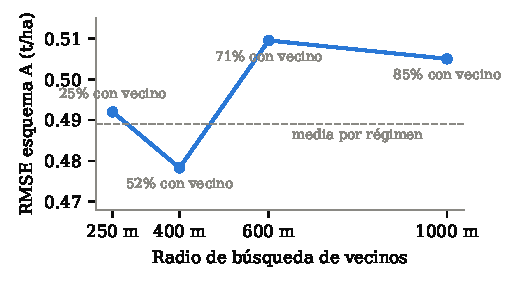
\includegraphics[width=\columnwidth]{f3_radio}
\caption{RMSE del modelo con régimen y rezago según el radio de búsqueda de vecinos. El texto indica qué fracción de
parcelas tiene al menos un vecino del mismo régimen.}
\label{fig:radio}
\end{figure}

\textbf{Otras dos decisiones.} Limitamos los vecinos al mismo régimen porque sus etiquetas se miden distinto. Como los
dos regímenes están en zonas separadas, a 400\,m el resultado es idéntico con o sin esa restricción, y la conservamos
como protección. Además, el modelo ve solo el valor del rezago y no el número de vecinos ni la distancia al más
cercano. Esas dos columnas extra agregaban ruido, y quitarlas bajó el RMSE de 0.478 a 0.470. Con ese cambio el
rezago ganó en 9 de 10 repeticiones, y fue la primera versión del rezago que lo logró.

\textbf{Prueba de permutación del rezago.} Para saber si la posición de los vecinos aporta, revolvimos las coordenadas
de las parcelas dentro de cada régimen y dejamos intactos el régimen y el rendimiento. Después recalculamos el rezago y
repetimos la validación, con 50 permutaciones y 3 repeticiones cada una. Esta prueba destruye a propósito la estructura
espacial. Si el rezago solo captara el nivel del régimen, el modelo con coordenadas revueltas predeciría igual de bien.
Ninguna de las 50 permutaciones igualó el error real, lo que da $p=0.02$, el valor más pequeño posible con 50 sorteos.
Con 200 permutaciones obtuvimos $p=0.01$ al revolver dentro del régimen y $p=0.005$ al revolver dentro del municipio.
Con 50 permutaciones dentro del municipio el resultado sigue siendo $p=0.02$. La prueba muestra que la posición de los
vecinos contiene información sobre el rendimiento además del régimen. No demuestra por sí sola que esta versión del
rezago sea mejor que otras, para eso usamos la comparación entre repeticiones.

\subsection{Variables satelitales, de clima y de topografía}\label{sec:bloques}
Sobre el modelo con régimen y rezago probamos cada bloque de variables por separado (Fig.~\ref{fig:bloques}). Ninguno
cumplió la regla. El que más se acercó fue la heterogeneidad del NDVI dentro de la parcela, que ganó en 7 de 10
repeticiones por 0.002\,t/ha, pero al revolver sus valores el modelo predijo igual ($p=0.63$). Juntar todos los
bloques satelitales empeoró el error a 0.498, porque con 138 parcelas el modelo empieza a aprender ruido. El clima
viene en celdas de unos 5\,km~\cite{funk2015,verdin2020}, así que solo distingue zonas, y eso ya lo hacen el régimen y los vecinos. También
empeoró el esquema B hasta 0.540. Por estas razones el modelo final no usa estas variables.

\begin{figure}[t]
\centering
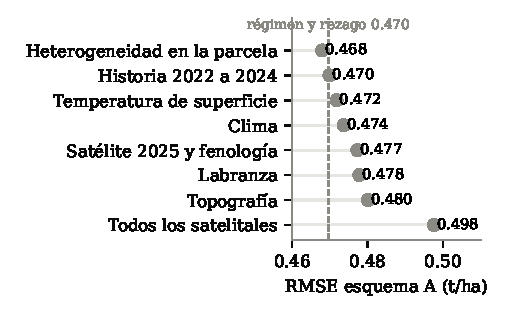
\includegraphics[width=\columnwidth]{f4_bloques}
\caption{RMSE al agregar cada bloque al modelo con régimen y rezago (línea punteada). Ninguno mejora de forma que
pase la regla de decisión.}
\label{fig:bloques}
\end{figure}

\subsection{Algoritmo}
Con las entradas fijas, régimen y rezago, comparamos algoritmos (Fig.~\ref{fig:algoritmos}). Los modelos de árboles,
bosque aleatorio y LightGBM, quedan peor que la media por régimen. Con solo tres entradas y 138 parcelas sus cortes
escalonados no tienen dónde apoyarse. Los modelos lineales, ridge, elastic net y PLS, quedan alrededor de 0.470. El
proceso gaussiano logra el menor error, 0.458, y gana al ridge en 9 de 10 repeticiones.

\begin{figure}[t]
\centering
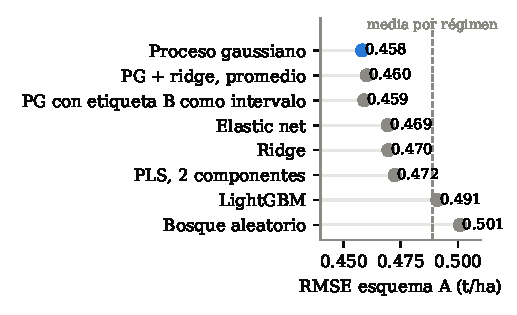
\includegraphics[width=\columnwidth]{f5_algoritmos}
\caption{RMSE de cada algoritmo con régimen y rezago. En gris, las alternativas. Las dos filas debajo del proceso
gaussiano (PG) son variantes que lo combinan con otras ideas.}
\label{fig:algoritmos}
\end{figure}

Elegimos el proceso gaussiano por tres razones además de su error. Primero, puede ajustar una relación suave y no
lineal entre el rezago y el rendimiento, mientras que un modelo lineal supone que cada t/ha de los vecinos pesa
igual en todo el rango. Segundo, tiene
pocos parámetros, tres en el kernel, que se ajustan con las propias parcelas, lo que busca limitar el sobreajuste con
muestras chicas. No lo damos por hecho y mostramos evidencia de estabilidad. El RMSE por repetición va de 0.442 a 0.503,
con desviación estándar de 0.018, y el proceso gaussiano gana a la media por régimen en 9 de 10 repeticiones. Con otras
cinco semillas de partición el promedio va de 0.452 a 0.468. Calculando el rezago sin la propia parcela, el error en el
entrenamiento de cada fold es 0.434 y el error en su fold de prueba es 0.450, una brecha de 0.016\,t/ha. Tercero, su
término de ruido absorbe parte del ruido de las etiquetas declaradas. Los procesos gaussianos ya se han usado para
predecir rendimiento con datos satelitales~\cite{you2017}.

Debemos matizar la ventaja del proceso gaussiano. Frente a un modelo lineal con las mismas entradas, la diferencia de
RMSE es de $-0.012$\,t/ha (intervalo de confianza del 95\,\% de $-0.039$ a $+0.015$, $p=0.38$), así que no lo supera de
forma significativa. Su ventaja clara es sobre los modelos de árboles.

\textbf{Ideas que no mejoraron al proceso gaussiano.} Promediarlo con un ridge (0.460) no ayudó, porque ambos usan la
misma información. Tratar la etiqueta del régimen B como un intervalo de $\pm0.25$\,t/ha para reflejar el redondeo
tampoco (0.459). Ponderar las parcelas por su área o usar una pérdida robusta de Huber mejoró menos de 0.004\,t/ha a
un ridge, sin superar al proceso gaussiano.

\section{Modelo final}\label{sec:final}

\subsection{Arquitectura}
El modelo recibe tres entradas por parcela, el régimen codificado en dos columnas indicadoras (A o B) y el rezago
espacial estandarizado. Un proceso gaussiano~\cite{rasmussen2006} predice el rendimiento suponiendo que parcelas con
entradas parecidas tienen rendimientos parecidos. Qué tan parecidas lo define la covarianza
\begin{equation}
k(\mathbf{x},\mathbf{x}') = \sigma_f^2 \exp\!\left(-\frac{\lVert\mathbf{x}-\mathbf{x}'\rVert^2}{2\lambda^2}\right) +
\sigma_n^2\,\delta_{\mathbf{x}\mathbf{x}'} ,
\label{eq:kernel}
\end{equation}
donde $\lambda$ es la distancia a la que dos parcelas dejan de parecerse, $\sigma_f^2$ la variación que explica el
modelo y $\sigma_n^2$ el ruido que no explica. Los tres se ajustan maximizando la verosimilitud. Dentro de
la validación se reajustan en cada fold usando solo las parcelas de entrenamiento de ese fold. En los 50 folds de
validación varían entre 0.51 y 1.41 para $\sigma_f^2$, entre 0.87 y 2.62 para $\lambda$ y entre 0.21 y 0.35 para
$\sigma_n^2$, sin tocar las cotas permitidas. El modelo final, que se entrega para predecir las 59 parcelas, se ajusta
con las 138 parcelas y queda con $\sigma_f^2=0.77$, $\lambda=1.57$ y $\sigma_n^2=0.26$, en unidades del rendimiento
estandarizado. Es decir, el modelo atribuye cerca de una cuarta parte de la variación a ruido. Lo que sí elegimos
viendo las 138 parcelas es la estructura del modelo, como el radio de 400\,m, los 10 vecinos y el algoritmo. El costo de
esa elección lo mide la validación anidada de la Sección~\ref{sec:confiabilidad}.

\subsection{Error de predicción}
En el esquema A el modelo obtiene un RMSE de 0.458\,t/ha, un error absoluto medio de 0.312 y un $R^2$ de 0.71. Mejora a
la media por régimen en los dos regímenes, de 0.535 a 0.494 en el A y de 0.398 a 0.389 en el B. En el esquema B empata
con ella (0.489), como se espera, porque sin vecinos cercanos el rezago se convierte en la media del régimen.

La Fig.~\ref{fig:obspred} muestra la limitación principal. Las predicciones forman dos franjas, una por régimen, y
dentro de cada una varían poco. Su desviación es cerca de 0.4 veces la de las etiquetas. El modelo acierta el nivel del
régimen y corrige con los vecinos, pero las parcelas con rendimientos extremos, como las de 5.5\,t/ha en
Chignahuapan, quedan cerca de la media. No forzamos más dispersión, porque sin información que la respalde subiría el
error.

\begin{figure}[t]
\centering
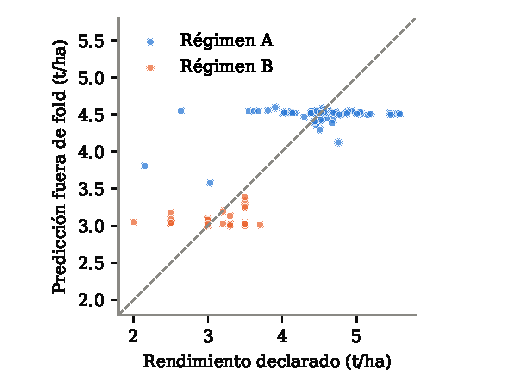
\includegraphics[width=0.9\columnwidth]{f6_observado_predicho}
\caption{Rendimiento declarado contra predicción fuera de fold, promedio de las 10 repeticiones. La línea punteada es
la predicción perfecta.}
\label{fig:obspred}
\end{figure}

\subsection{Intervalos de predicción}
Para FIRA, que evalúa crédito, importa también cuánto puede fallar cada predicción. Cada parcela recibe un intervalo
del percentil 10 al 90 calculado con predicción conformal dividida~\cite{vovk2005,lei2018}, en su variante de Mondrian,
que calibra por separado en cada grupo, aquí cada régimen~\cite{vovk2005}. El método tiene tres pasos. Primero,
guardamos los errores con signo $r=y-\hat y$ de las predicciones fuera de fold, es decir, de parcelas que el modelo no
vio, en las 10 repeticiones de la validación cruzada. Son 1380 errores, 870 del régimen A y 510 del B. Segundo, para cada
régimen calculamos los cuantiles 0.10 y 0.90 de sus errores. En el A valen $-0.51$ y $+0.57$, y en el B $-0.55$ y
$+0.48$\,t/ha. Tercero, el intervalo de una parcela es p10 igual a la predicción más el cuantil 0.10 de su régimen, y
p90 igual a la predicción más el cuantil 0.90. Como los cuantiles tienen signo, el intervalo no es simétrico. Los 1380
errores son 138 parcelas repetidas 10 veces, así que la calibración equivale a 87 parcelas en el A y 51 en el B. Con los
mismos errores estimamos la probabilidad de que el rendimiento quede por debajo de 2.5\,t/ha.

Para medir si el intervalo cumple, usamos validación anidada, en la que la parcela evaluada no participa ni en el
ajuste ni en la calibración (Fig.~\ref{fig:cobertura}). La cobertura total es 0.826, que son 570 aciertos en 690
evaluaciones (138 parcelas por 5 repeticiones), con un ancho medio de 1.13\,t/ha. Como cada parcela se evalúa cinco
veces, calculamos el intervalo de confianza del 95\,\% con un bootstrap por parcela y resulta de 0.765 a 0.883, que
incluye la meta de 0.80. Por régimen la cobertura es 0.791 en el A (intervalo de 0.708 a 0.869) y 0.886 en el B
(de 0.816 a 0.949). En el cuartil de parcelas más chicas es 0.77 (de 0.63 a 0.90). Con 35 parcelas por cuartil, esta
diferencia no es concluyente y la tratamos solo como una observación exploratoria.

\begin{figure}[t]
\centering
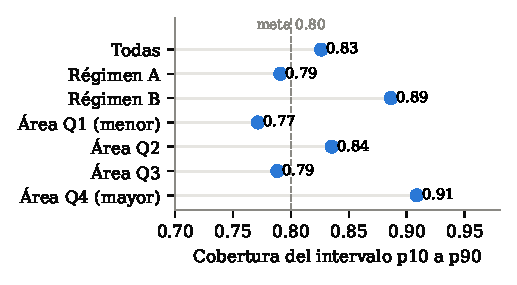
\includegraphics[width=\columnwidth]{f10_cobertura}
\caption{Fracción de parcelas cuyo rendimiento cae dentro de su intervalo p10 a p90, por régimen y por cuartil de
área. La meta es 0.80.}
\label{fig:cobertura}
\end{figure}

\subsection{Predicciones de las 59 parcelas}
El Cuadro~\ref{tab:predicciones} del apéndice lista las 59 predicciones con sus intervalos. Las 37 parcelas del régimen A tienen una predicción media de 4.49\,t/ha (de 3.72 a 4.58) y las 22 del B de 3.06\,t/ha
(de 2.75 a 3.66), igual que las medias de entrenamiento (Fig.~\ref{fig:mapa}). Ninguna sale del rango observado en
su régimen. La probabilidad de quedar bajo 2.5\,t/ha supera 0.10 en 18 parcelas, todas del régimen B.

\begin{figure}[t]
\centering
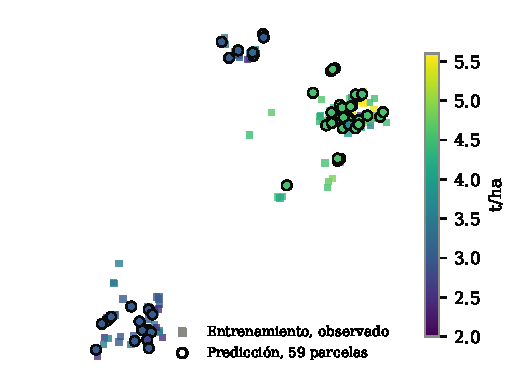
\includegraphics[width=0.95\columnwidth]{f12_mapa}
\caption{Rendimiento observado en las parcelas de entrenamiento (cuadros) y predicho en las 59 parcelas (círculos con
borde), con la misma escala de color. Los grupos en tonos oscuros, al oeste, son del régimen B.}
\label{fig:mapa}
\end{figure}

\section{Qué tan confiable es el error}\label{sec:confiabilidad}

Un RMSE de validación cruzada no es todavía el error que tendremos en las 59 parcelas. Revisamos tres cosas.

\textbf{¿La mejora es real o es azar?} La Fig.~\ref{fig:repeticiones} muestra el RMSE de cada una de las 10
repeticiones. El proceso gaussiano gana a la media por régimen y al ridge en 9 de 10. Pero las repeticiones usan las
mismas 138 parcelas, así que no son independientes y contar victorias exagera la evidencia. Con la prueba $t$
corregida de Nadeau y Bengio~\cite{nadeau2003}, la ventaja sobre la media por régimen es de 0.029\,t/ha, con un
intervalo de confianza del 95\,\% de $-0.079$ a $0.022$ ($p=0.26$). La dirección es consistente, pero con 138
parcelas la mejora no alcanza a ser significativa.

\begin{figure}[t]
\centering
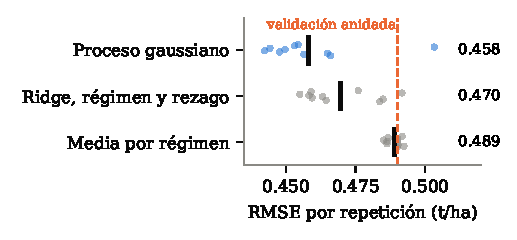
\includegraphics[width=\columnwidth]{f7_repeticiones}
\caption{RMSE de cada repetición del esquema A (puntos) y su promedio (barra). La línea naranja es el error estimado
con validación anidada.}
\label{fig:repeticiones}
\end{figure}

\textbf{¿Cuánto infla el resultado haber elegido el mejor?} Probamos decenas de variantes con las mismas particiones
y nos quedamos con la mejor, lo que favorece a la que tuvo suerte en esas particiones~\cite{cawley2010}. La validación
anidada lo corrige~\cite{varma2006}. En cada fold externo repetimos la elección entre 12 variantes usando solo las
parcelas de entrenamiento, y evaluamos la elegida en el fold externo. El resultado es 0.490\,t/ha, igual que la media
por régimen. La elección interna se repartió entre la media por régimen (6 de 15 folds) y el proceso gaussiano con
rezago a 400\,m (6 de 15). Cambiando la semilla de las particiones, el proceso gaussiano obtiene entre 0.452 y 0.468.
Por eso esperamos un RMSE de 0.46 a 0.49\,t/ha. Las 59 parcelas tienen algo más de vecinos que las de validación
(61\,\% con un vecino a 400\,m o menos, contra 46\,\%), así que el extremo bajo es plausible.

\textbf{¿Hay fuga de información?} Si la etiqueta se filtrara a las variables, el modelo predeciría bien aunque las
etiquetas no tuvieran sentido. Lo probamos revolviendo los rendimientos dentro de cada régimen, lo que conserva el
régimen pero rompe la relación con los vecinos (Fig.~\ref{fig:permutacion}). Con las etiquetas revueltas el modelo
nunca baja de 0.488, y con las reales obtiene 0.467 en las mismas condiciones. Revolviendo entre todas las parcelas, el
modelo queda en 0.861, peor que la media global (0.855). El rezago capta una relación real entre vecinos.

\begin{figure}[t]
\centering
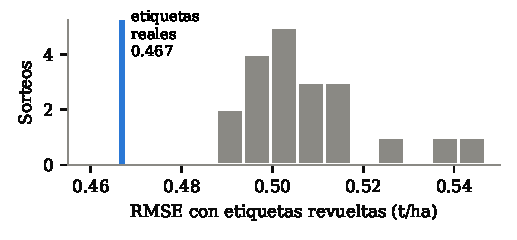
\includegraphics[width=\columnwidth]{f8_permutacion}
\caption{RMSE del modelo en 20 sorteos con los rendimientos revueltos dentro de cada régimen, contra el RMSE con los
rendimientos reales.}
\label{fig:permutacion}
\end{figure}

\textbf{Margen por calificar con 59 parcelas.} Aun con el modelo correcto, el RMSE de 59 parcelas varía según cuáles
toquen. Sorteamos 5000 grupos de 37 errores del régimen A y 22 del B, como en la partición oficial
(Fig.~\ref{fig:margen}). El 90\,\% de los sorteos cae entre 0.35 y 0.56\,t/ha. Este margen es mayor que la diferencia
entre cualquiera de los modelos que comparamos.

\begin{figure}[t]
\centering
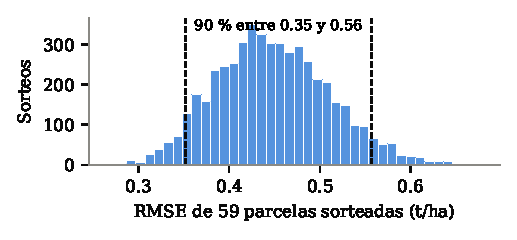
\includegraphics[width=\columnwidth]{f9_margen}
\caption{RMSE de 5000 grupos de 59 parcelas sorteados entre los errores fuera de fold del modelo.}
\label{fig:margen}
\end{figure}

\section{Qué aportan los índices satelitales}\label{sec:indices}

El reto pregunta qué índice y qué variable climática pesan más. Para responder usamos un bosque aleatorio de análisis,
que aprovecha muchas variables, y medimos cuánto sube su RMSE al revolver los valores de cada índice. Lo hicimos en dos
escenarios (Fig.~\ref{fig:indices}).

\begin{figure}[t]
\centering
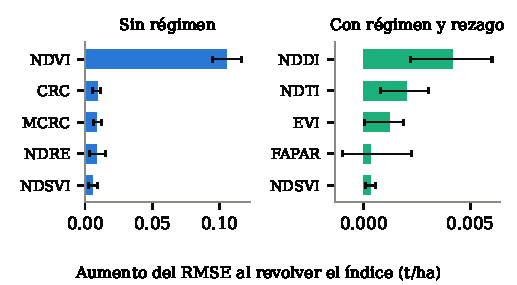
\includegraphics[width=\columnwidth]{f11_indices}
\caption{Aumento del RMSE al revolver cada índice, con su intervalo entre repeticiones. Nótese que las escalas
horizontales son distintas.}
\label{fig:indices}
\end{figure}

Sin el régimen, el NDVI es por mucho el más importante. Revolverlo sube el RMSE 0.106\,t/ha. Pero el NDVI histórico de
cada parcela distingue las zonas y con ellas el régimen, así que en buena parte funciona como un sustituto del
régimen. El modelo solo con variables satelitales llega a 0.696\,t/ha, muy lejos de 0.489 de la media por régimen. Lo
mismo pasa con la lluvia, que sin el régimen sube el RMSE 0.364\,t/ha porque sus celdas de 5\,km identifican la zona.

Con el régimen y el rezago presentes, el índice de sequía NDDI es el que más aporta, pero solo 0.004\,t/ha, y ninguna
variable climática aporta. Es plausible que el NDDI importe, porque marca las parcelas que se secaron o se acamaron
antes en un año muy lluvioso. Aun así, su efecto es mucho menor que el margen de azar de la
Sección~\ref{sec:confiabilidad}. Esta es la razón de fondo por la que el modelo final no usa satélite. Con etiquetas
declaradas y ruidosas, la información de las imágenes queda por debajo del ruido.

\section{Conclusiones}\label{sec:conclusiones}

El modelo final es deliberadamente simple. Usa el régimen de la etiqueta, que explica la mayor parte del error que se
puede reducir, y el rendimiento de los vecinos del mismo régimen a 400\,m, combinados con un proceso gaussiano. Cada
pieza entró porque mejoró la validación de forma consistente y pasó una prueba de permutación, y cada pieza que se
quedó fuera, como las variables satelitales y climáticas o los modelos de árboles, lo hizo porque no mejoró. El
modelo obtiene 0.458\,t/ha en validación cruzada, y estimamos un RMSE de 0.46 a 0.49\,t/ha en las 59 parcelas, con un
margen adicional por el tamaño de la muestra de calificación.

La lección principal es que en este reto el límite no lo pone el algoritmo sino las etiquetas. Con dos formas de
reportar y rendimientos declarados, la mejora sobre la media por régimen es pequeña y cualquier variable adicional
compite contra el ruido. Mejores datos de campo, como el rendimiento medido o la fecha de siembra, ayudarían más que
un modelo más complejo.


% Sólo las referencias citadas en el texto, en estilo IEEE y en orden de aparición.
\begin{thebibliography}{99}

\bibitem{sader2025}
Secretaría de Agricultura y Desarrollo Rural, ``Del campo a la copa: el recorrido de la cebada,'' \emph{gob.mx}, 11 de noviembre de 2025. [En línea]. Disponible: \url{https://www.gob.mx/agricultura/articulos/del-campo-a-la-copa-el-recorrido-de-la-cebada}

\bibitem{drusch2012}
M. Drusch \emph{et al.}, ``Sentinel-2: ESA's Optical High-Resolution Mission for GMES Operational Services,'' \emph{Remote Sensing of Environment}, vol.~120, pp.~25--36, 2012.

\bibitem{frazier2021}
A.~E. Frazier y B.~L. Hemingway, ``A Technical Review of Planet Smallsat Data: Practical Considerations for Processing and Using PlanetScope Imagery,'' \emph{Remote Sensing}, vol.~13, no.~19, p.~3930, 2021.

\bibitem{funk2015}
C. Funk \emph{et al.}, ``The climate hazards infrared precipitation with stations---a new environmental record for monitoring extremes,'' \emph{Scientific Data}, vol.~2, art.~150066, 2015.

\bibitem{verdin2020}
A. Verdin \emph{et al.}, ``Development and validation of the CHIRTS-daily quasi-global high-resolution daily temperature data set,'' \emph{Scientific Data}, vol.~7, no.~1, art.~303, 2020.

\bibitem{vanklompenburg2020}
T. van Klompenburg, A. Kassahun y C. Catal, ``Crop yield prediction using machine learning: A systematic literature review,'' \emph{Computers and Electronics in Agriculture}, vol.~177, p.~105709, 2020.

\bibitem{weiss2020}
M. Weiss, F. Jacob y G. Duveiller, ``Remote sensing for agricultural applications: A meta-review,'' \emph{Remote Sensing of Environment}, vol.~236, p.~111402, 2020.

\bibitem{lobell2020}
D.~B. Lobell \emph{et al.}, ``Eyes in the Sky, Boots on the Ground: Assessing Satellite‐ and Ground‐Based Approaches to Crop Yield Measurement and Analysis,'' \emph{American Journal of Agricultural Economics}, vol.~102, no.~1, pp.~202--219, 2020.

\bibitem{zadoks1974}
J.~C. Zadoks, T.~T. Chang y C.~F. Konzak, ``A decimal code for the growth stages of cereals,'' \emph{Weed Research}, vol.~14, no.~6, pp.~415--421, 1974.

\bibitem{roberts2017}
D.~R. Roberts \emph{et al.}, ``Cross-validation strategies for data with temporal, spatial, hierarchical, or
phylogenetic structure,'' \emph{Ecography}, vol.~40, no.~8, pp.~913--929, 2017.

\bibitem{ploton2020}
P. Ploton \emph{et al.}, ``Spatial validation reveals poor predictive performance of large-scale ecological mapping models,'' \emph{Nature Communications}, vol.~11, no.~1, art.~4540, 2020.

\bibitem{ojala2010}
M.~Ojala y G.~C. Garriga, ``Permutation tests for studying classifier performance,'' \emph{Journal of Machine
Learning Research}, vol.~11, pp.~1833--1863, 2010.

\bibitem{benjamini1995}
Y. Benjamini y Y. Hochberg, ``Controlling the False Discovery Rate: A Practical and Powerful Approach to Multiple Testing,'' \emph{Journal of the Royal Statistical Society Series B: Statistical Methodology}, vol.~57, no.~1, pp.~289--300, 1995.

\bibitem{cawley2010}
G.~C. Cawley y N.~L.~C. Talbot, ``On over-fitting in model selection and subsequent selection bias in performance
evaluation,'' \emph{Journal of Machine Learning Research}, vol.~11, pp.~2079--2107, 2010.

\bibitem{varma2006}
S.~Varma y R.~Simon, ``Bias in error estimation when using cross-validation for model selection,'' \emph{BMC
Bioinformatics}, vol.~7, art.~91, 2006.

\bibitem{nadeau2003}
C.~Nadeau e Y.~Bengio, ``Inference for the generalization error,'' \emph{Machine Learning}, vol.~52, no.~3,
pp.~239--281, 2003.

\bibitem{kaufman2012}
S.~Kaufman, S.~Rosset, C.~Perlich y O.~Stitelman, ``Leakage in data mining: Formulation, detection, and
avoidance,'' \emph{ACM Transactions on Knowledge Discovery from Data}, vol.~6, no.~4, art.~15, 2012.

\bibitem{tobler1970}
W.~R. Tobler, ``A computer movie simulating urban growth in the Detroit region,'' \emph{Economic Geography},
vol.~46, pp.~234--240, 1970.

\bibitem{you2017}
J. You \emph{et al.}, ``Deep Gaussian Process for Crop Yield Prediction Based on Remote Sensing Data,'' \emph{Proceedings of the AAAI Conference on Artificial Intelligence}, vol.~31, no.~1, 2017.

\bibitem{rasmussen2006}
C.~E. Rasmussen y C.~K.~I. Williams, \emph{Gaussian Processes for Machine Learning}. Cambridge, MA, EE.~UU.: MIT
Press, 2006.

\bibitem{vovk2005}
V.~Vovk, A.~Gammerman y G.~Shafer, \emph{Algorithmic Learning in a Random World}. Nueva York, NY, EE.~UU.:
Springer, 2005.

\bibitem{lei2018}
J. Lei \emph{et al.}, ``Distribution-Free Predictive Inference for Regression,'' \emph{Journal of the American Statistical Association}, vol.~113, no.~523, pp.~1094--1111, 2018.

\bibitem{gu2007}
Y. Gu \emph{et al.}, ``A five‐year analysis of MODIS NDVI and NDWI for grassland drought assessment over the central Great Plains of the United States,'' \emph{Geophysical Research Letters}, vol.~34, no.~6, art.~2006GL029127, 2007.

\bibitem{samarah2005}
N.~H. Samarah, ``Effects of drought stress on growth and yield of barley,'' \emph{Agronomy for Sustainable Development}, vol.~25, no.~1, pp.~145--149, 2005.

\bibitem{passarella2002}
V.~S. Passarella, R. Savin y G.~A. Slafer, ``Grain weight and malting quality in barley as affected by brief periods of increased spike temperature under field conditions,'' \emph{Australian Journal of Agricultural Research}, vol.~53, no.~11, pp.~1219--1227, 2002.

\end{thebibliography}

\end{document}
